%Problem Set 2
%%%%%%%%%%%%%%%%%%%%%%%%%%%%%%%%%%%%%%%%%%%%%%%%

%Sweave('C:/Klaus/AAEC5126/problemsets/ps4',syntax=SweaveSyntaxNoweb)

%I) DEFINE DOCUMENTCLASS AND LOAD ALL REQUIRED PACKAGES
\documentclass[11pt,reqno]{amsart}\usepackage[]{graphicx}\usepackage[]{color}
% maxwidth is the original width if it is less than linewidth
% otherwise use linewidth (to make sure the graphics do not exceed the margin)
\makeatletter
\def\maxwidth{ %
  \ifdim\Gin@nat@width>\linewidth
    \linewidth
  \else
    \Gin@nat@width
  \fi
}
\makeatother

\definecolor{fgcolor}{rgb}{0.196, 0.196, 0.196}
\newcommand{\hlnum}[1]{\textcolor[rgb]{0.063,0.58,0.627}{#1}}%
\newcommand{\hlstr}[1]{\textcolor[rgb]{0.063,0.58,0.627}{#1}}%
\newcommand{\hlcom}[1]{\textcolor[rgb]{0.588,0.588,0.588}{#1}}%
\newcommand{\hlopt}[1]{\textcolor[rgb]{0.196,0.196,0.196}{#1}}%
\newcommand{\hlstd}[1]{\textcolor[rgb]{0.196,0.196,0.196}{#1}}%
\newcommand{\hlkwa}[1]{\textcolor[rgb]{0.231,0.416,0.784}{#1}}%
\newcommand{\hlkwb}[1]{\textcolor[rgb]{0.627,0,0.314}{#1}}%
\newcommand{\hlkwc}[1]{\textcolor[rgb]{0,0.631,0.314}{#1}}%
\newcommand{\hlkwd}[1]{\textcolor[rgb]{0.78,0.227,0.412}{#1}}%
\let\hlipl\hlkwb

\usepackage{framed}
\makeatletter
\newenvironment{kframe}{%
 \def\at@end@of@kframe{}%
 \ifinner\ifhmode%
  \def\at@end@of@kframe{\end{minipage}}%
  \begin{minipage}{\columnwidth}%
 \fi\fi%
 \def\FrameCommand##1{\hskip\@totalleftmargin \hskip-\fboxsep
 \colorbox{shadecolor}{##1}\hskip-\fboxsep
     % There is no \\@totalrightmargin, so:
     \hskip-\linewidth \hskip-\@totalleftmargin \hskip\columnwidth}%
 \MakeFramed {\advance\hsize-\width
   \@totalleftmargin\z@ \linewidth\hsize
   \@setminipage}}%
 {\par\unskip\endMakeFramed%
 \at@end@of@kframe}
\makeatother

\definecolor{shadecolor}{rgb}{.97, .97, .97}
\definecolor{messagecolor}{rgb}{0, 0, 0}
\definecolor{warningcolor}{rgb}{1, 0, 1}
\definecolor{errorcolor}{rgb}{1, 0, 0}
\newenvironment{knitrout}{}{} % an empty environment to be redefined in TeX

\usepackage{alltt}   %keep it simple
\usepackage{hyperref}
\usepackage{graphicx}      % for fancy graphics
\usepackage{setspace}      % for basic formatting
\usepackage{enumerate}     % for more flexibility with numbered lists
%\SweaveOpts{keep.source=TRUE}  %KEY - this preserves R formatting and comments

% You may need to load all or some of these packages -
%follow the instructions on our course web site under "Help with LaTex"

%II) PREAMBLE
%%%%%%%%%%%%%%%%%%%%%%%%%%%%%%%%%%%%%%%%%%%%%%%%%%
\pagestyle{plain} %puts page number center bottom
\setlength{\topmargin}{0in}
\setlength{\textheight}{8.5in}
\setlength{\oddsidemargin}{.0in}
\setlength{\evensidemargin}{.0in}
\setlength{\textwidth}{6.5in}
\setlength{\footskip}{.5in}
\setlength{\parindent}{0in} %suppress indentation
%\onehalfspacing

\newcommand{\mlt}[1]{\mathbf{#1}} %matrix bold for Latin symbols
\newcommand{\mgr}[1]{\mathbf{#1}}%matrix bold for Greek symbols
\newcommand{\kR}{\tt R\rm{} }%shortcut for "R" symbol
\newcommand{\ksp}{\vspace{0.1in}}   % insert some space between chunks
%feel free to add your own shortcuts  - here a mine:
\newcommand{\kl}{\left(}
\newcommand{\kr}{\right)}
\newcommand{\kll}{\left\{}
\newcommand{\krr}{\right\}}
\newcommand{\kmu}{\mgr{\mu}}
\newcommand{\kpsi}{\mgr{\psi}}
\newcommand{\kphi}{\mgr{\phi}}
\newcommand{\kgam}{\mgr{\gamma}}
\newcommand{\ktheta}{\mgr{\theta}}
\newcommand{\kbeta}{\mgr{\beta}}
\newcommand{\kdelta}{\mgr{\delta}}
\newcommand{\kt}{^{\prime}}
\newcommand{\kdel}{\partial}
\newcommand{\kdot}{\kl . \kr}
\newcommand{\keps}{\epsilon}
\newcommand{\kx}{\mlt{x}}
\newcommand{\kX}{\mlt{X}}
\newcommand{\kZ}{\mlt{Z}}
\newcommand{\kV}{\mlt{V}}
\newcommand{\kM}{\mlt{M}}
\newcommand{\kP}{\mlt{P}}
\newcommand{\ky}{\mlt{y}}
\newcommand{\kb}{\mlt{b}}
\newcommand{\kc}{\mlt{c}}
\newcommand{\ki}{\mlt{i}}
\newcommand{\ke}{\mlt{e}}
\newcommand{\klam}{\lambda}
\newcommand{\kp}{\mlt{p}}
\newcommand{\kprob}{\text{prob}}
\newcommand{\kz}{\mlt{z}}
\newcommand{\ksig}{\sigma^2}
\newcommand{\kSig}{\mgr{\Sigma}}
\newcommand{\klog}{\text{log}}
\newcommand{\kols}{\kl \kX\kt\kX\kr^{-1}\kX\kt\ky}
\newcommand{\kSSE}{\kl \ky-\kX\kb\kr\kt\kl\ky-\kX\kb\kr}

\newenvironment{nouppercase}{%
  \let\uppercase\relax%
  \renewcommand{\uppercasenonmath}[1]{}}{}
  
%%%%%%%%%%%%%%%%%%%%%%%%
\IfFileExists{upquote.sty}{\usepackage{upquote}}{}
\begin{document}
%\SweaveOpts{concordance=TRUE}
%%%%%%%%%%%%%%%%%%%%%%%%

%III) TOP MATTER INFORMATION
\title{Problem Set 4}
\author{Nima Mohammadi \\ \href{mailto:nimamo@vt.edu}{\textbf{nimamo@vt.edu}}} %ENTER YOUR NAME HERE
\begin{nouppercase}
\maketitle %this comes at the end of the top matter to set it.
\end{nouppercase}










%%%%%%%%%%%%%%%%%%%%%%%%%%%%%%%%%%%%%%%%%%%%%%%%%%%%%%%%%%%%%%%%%%%%%%%%
\section{Instrumental Variables/TSLS}
%%%%%%%%%%%%%%%%%%%%%%%%%%%%%%%%%%%%%%%%%%%%%%%%%%%%%%%%%%%%%%%%%%%%%%%%

Consider the following regression model: $h_{i}=\beta_{1} a g e_{i}+\beta_{2} e x_{i}+\varepsilon_{i}$ 

where $h_{i}$ is a (continuous) health index for professional worker $i$, $age_{i}$ is the age of worker $i$ and $ex_i$ is the hours of exercise per week for worker $i$. Assume all these (and subsequent variables) are expressed as deviations from their respective mean (So we don't have to worry about intercept terms, which will make the following a bit easier).  The full model can thus be written as 

$\mlt{h}=\mlt{X} \boldsymbol{\beta}+\boldsymbol{\varepsilon} \text { where } \quad \mlt{X}=\left[\begin{array}{lll}
\mlt{age} & \mlt{ex}
\end{array}\right] \text { and } \quad \boldsymbol{\beta}=\left[\begin{array}{l}
\beta_{1} \\
\beta_{2}
\end{array}\right]$


\ksp
\begin{enumerate}[(a)]
\item  Why might you suspect that exercise could be correlated with the error term? (provide some reasoning / intuition).\\


There are clearly many more variables that can potentially impacts on the health of the worker. For example, indivual dietary choice, smoking habits or the time that the worker spends working. That is there are many variables that are excluded which are exhibited in the error term. However, the time of the worker is partitioned between exercise and other activities that impacts his/her health, such as the time spent working per week. That is working hours in an omitted variable that is correlated with exercise and consequently we can conclude that the error term is correlated with the variable exercise.

\ksp
\item If this is the case (i.e $\operatorname{plim}\left(\frac{1}{n} \mlt{ex}^{\prime} \mlt{\varepsilon}\right)=\varphi \neq 0$) determine whether $b_{OLS}$ is a consistent estimator for $\kbeta$.\\

\begin{equation*}
\begin{split}
& \operatorname{plim} \mlt{b}=\kbeta+ \operatorname{plim} \left(\frac{1}{n} \kX\kt\kX\right)^{-1} \operatorname{plim} \left(\frac{1}{n} \mlt{X}^{\prime} \varepsilon\right)=\beta+\mlt{Q}_{\mlt{X} \mlt{X}}^{-1} p \lim \left[\begin{array}{c}
  \frac{1}{n}\bold{age}\kt\mgr{\varepsilon}  \\
  \frac{1}{n}\bold{ex}\kt\mgr{\varepsilon}  \\
\end{array}\right]=\kbeta+\mlt{Q}_{\mlt{X} \mlt{X}}^{-1}\left[\begin{array}{l}
\mgr{\gamma} \\
\mgr{\varphi}
\end{array}\right]\\
& \varphi\neq 0 \rightarrow \operatorname{plim}\bold{b}\neq \kbeta
\end{split}
\end{equation*}\\



That is $b_{OLS}$ is not a consistent estimator for $\kbeta$.

\ksp
\item Suppose you have information on all workers in your sample for two additional variables: "distance from home to nearest health club" $(dh_i)$, and "distance from work to nearest health club" $(dw_i)$.
Assume neither of these variables are correlated with $\mgr{\varepsilon}$ , i.e. $\operatorname{plim} (\bold{dh}\kt \mgr{\varepsilon} ) = \operatorname{plim} (\bold{dw}\kt \mgr{\varepsilon} ) = \mlt{0}$ . Why might these variables be good instruments for exercise?\\

For a good instrumental variable it should have two properties: i) noncorrelated with error term, and ii) highly correlated with troublemakers. 

The first condition is satisfied as this property is stated in the question. Also, they are highly correlated with the exercise time. Intuitively, being closer to the exercise club increases the frequency of going to the club and exercising. Hence, they are good IVs for exercise.\\

\ksp
\item Show how these additional variables can be used to derive a consistent TSLS estimator for $\kbeta$ (show all detailed steps). Proof that this estimator is indeed consistent. (Assume that $plim(\mlt{Z}\kt\mlt{Z}/n) = \bold{Q}_\bold{zz}$ and $\operatorname{plim}(\mlt{Z}\kt\kX/n) = \bold{Q}_\bold{zx}$ are well-behaved finite matrices.)\\


\begin{equation*}
\begin{split}
\operatorname{plim}\bold{b}_{TSLS} &= \operatorname{plim}\left[\left(\hat{\mlt{X}}^{\prime} \hat{\mlt{X}}\right)^{-1} \hat{\mlt{X}}^{\prime} \mlt{y}\right] = \operatorname{plim}[(\kX\kt\kZ(\kZ\kt\kZ)^{-1}\kZ\kt\kX)^{-1}\kX\kt\kZ(\kZ\kt\kZ)^{-1}\kZ\kt\ky]\\
&= \operatorname{plim} [(\kX\kt\kZ(\kZ\kt\kZ)^{-1}\kZ\kt\kX)^{-1}\kX\kt\kZ(\kZ\kt\kZ)^{-1}\kZ\kt(\kX\kbeta+\mgr{\varepsilon})]
\end{split}
\end{equation*}
\begin{equation*}
\begin{split}
\Rightarrow \operatorname{plim} \bold{b}_{TSLS}=\kbeta + (\bold{Q}\kt_{\mlt{Z}\kX}(\bold{Q}_{\mlt{Z}\mlt{Z}})^{-1}\bold{Q}_{\mlt{Z}\kX})^{-1}\bold{Q}\kt_{\mlt{Z}\kX}(\bold{Q}_{\mlt{Z}\mlt{Z}})^{-1} \operatorname{plim}((1/n)\mlt{Z}\kt\mgr{\varepsilon})
\end{split}
\end{equation*}

Since the instrument is derived such that $COV(\mlt{Z}_i , \mgr{\varepsilon})=0$, so $\operatorname{plim}(\frac{1}{n}\mlt{Z}\kt\mgr{\varepsilon})=0$ Then we have
$\operatorname{plim} \bold{b}_{TSLS}=\kbeta$
which is a consistent estimator.\\

\item What would you use for a consistent estimator for $\sigma^{2}$ ? (show detailed expression)
\ksp

The Asymptotic variance  of $\kb_{TSLS}$ can be estimated by:
\begin{equation*}
\begin{split}
& \hat{\mlt{V}}_a(\kb_{TSLS})=\hat{\sigma}^2 (\kX'\mlt{Z}(\mlt{Z}'\mlt{Z})^{ - 1} \mlt{Z}'\kX)^{ - 1} 
\end{split}
\end{equation*}
$\hat{\sigma}^2$ is estimator for ${\sigma}^2$ and can be derived as:
\begin{equation*}
\begin{split}
& \hat{\sigma}^2=\frac{{\hat{\mgr{\varepsilon}} '\hat{\mgr{\varepsilon} }}}{n}
\end{split}
\end{equation*}
where residuals, $\hat{\mgr{\varepsilon}}$, can be derived as:
\begin{equation*}
\begin{split}
& \hat{\mgr{\varepsilon}}=\ky - \kX \kb_{TSLS}
\end{split}
\end{equation*}
Needless to say the original $\kX$ is used in the computation of the residuals. \\

\item Outline in detail how a Hausman test and a Wu test could be performed to test $H_0:\varphi= 0$\\

The Hausman test is a type of Wald test which examines if the difference between 2 sets of estimates arise from 2 different models, weighted by the difference in their asymptotic variance-covariance
matrix, is "large enough" to reject the null hypothesis that they are the same.

The rationale is that the first model considered is known to generate consistent estimates under OV-type problems or other mis-specification issues, while the second model is inconsistent if there are indeed OV
type problems or mis-specifications. However, the first estimator is always less efficient than the second. So if there are no OV-type or mis-specification problems, it would be better to choose the second model.
If there are OV type problems, we should use the first model (since consistency is generally more important than efficiency). 

For the case at hand, the IV (or TSLS) model is "model 1" - consistent under OV-problems, however it is less efficient. The OLS model is "model 2" - more efficient, but inconsistent under OV-problems. The H-test
examines if the two estimators are "close enough" to conclude that OLS is fine, i.e. that there are no OV type problems (the null hypothesis). If the weighted difference between the estimators is "too
large", the test would reject the null.
The H-test statistic is thus derived as:

\begin{equation*}
\begin{split}
&  H = \mlt{d}'(\hat V_a (\mlt{b}_{TSLS} ) - \hat V_a (\mlt{b_{OLS}}))^{ - 1} \mlt{d} = \mlt{d}'(s^2 (\hat \kX'\hat \kX)^{-1}  - s^2 (\kX'\kX)^{ - 1} )^{ - 1} \mlt{d} \sim \chi ^2 (J)   
\end{split}
\end{equation*}
where $\mlt{d} = (\mlt{b_{TSLS}}  - \kb_{OLS})$, $\hat {\kX} = \mlt{Z}(\mlt{Z}'\mlt{Z})^{ - 1} \mlt{Z}'\kX$, $s^2  = \frac{{\ke'\ke}}{{n - k}}$.\\


When we fail to reject the null we mean that the difference between the estimators are not too large, and since TSLS gives consistent estimates, $\mlt{b_{TSLS}}  = \kb_{OLS}$ are consistent. Since $\kb_{OLS}$ is consistent  using equation 1 we must have:  
\begin{equation*}
\begin{split}
& \operatorname{plim} \kb = \kbeta \Rightarrow \mlt{Q_{XX}}^{ - 1} \left[ {\begin{array}{*{20}c}
   \mgr{\gamma}   \\
   \mgr{\varphi}   \\
\end{array}} \right] = \mlt{0} \Rightarrow \mgr{\gamma}=0 \mbox{ and } \mgr{\varphi}=0
\end{split}
\end{equation*}
Therefore we can test $H_0 :  \mgr{\varphi} = 0$ with Hausman test and when we fail to reject the "Hausman test null" we fail to reject $H_0$ too. In addition, when we reject the "Hausman test null" we can claim that "either $\mgr{\gamma} \neq 0$ or $ \mgr{\varphi} \neq 0$ or both". In that case the alternative hypothesis is \textit{not} $H_1: \mgr{\varphi} \neq 0$. Even in this case we might have $\mgr{\varphi} =0$.  

"Wu test" is an equivalent test that avoids the inverse problem of the Hausman test. we know that a rejection of the null hypothesis would reveal Omitted Variable problems in the OLS model. This  suggests that we should follow an IV approach. On the other hand if the null is not rejected, the OLS is fine. As in the case of the Hausman test, when we fail to reject the "Wu test null" we fail to reject $H_0 :  \mgr{\varphi} = 0$ but if we reject "Wu test null" we can just say that "either $\mgr{\gamma} \neq 0$ or $ \mgr{\varphi} \neq 0$ or both".  
\end{enumerate}


%%%%%%%%%%%%%%%%%%%%%%%%%%%%%%%%%%%%%%%%%%%%%%%%%%%%%%%%%%%%%%%%%%%%%%%%
\section{Instrumental Variables and Specification Tests in \kR}
%%%%%%%%%%%%%%%%%%%%%%%%%%%%%%%%%%%%%%%%%%%%%%%%%%%%%%%%%%%%%%%%%%%%%%%%

Use Greene's quarterly macroeconomic data (data set "consumption” on our course web site).


Consider the model  


$y_{t}=\beta_{0}+\beta_{1} dpi_{t}+\beta_{2} cpi_{t}+\beta_{3} \text {rate}_{t}+\varepsilon_{t}$

where \\
$t$ indexes the current time period, \\
$y=$ aggregate consumption (billion dollars, denoted as "realcons" in the variable list),\\
$dpi=$ aggregate disposable income ("realdpi" in the list), \\
$cpi=$ consumer price index, and \\
$rate$ = real interest rate ("realint" in the list).

You suspect that $dpi$ is correlated with the error term for the same time period. You decide to instrument it with $dpi$, and $y_{t-1}$, i.e. lagged dpi and lagged consumption.

Use the procedure outlined in script \texttt{mod4s1bto} generate all needed lagged variables.

\begin{knitrout}
\definecolor{shadecolor}{rgb}{1, 1, 1}\color{fgcolor}\begin{kframe}
\begin{alltt}
\hlstd{data} \hlkwb{<-} \hlkwd{read.table}\hlstd{(}\hlstr{'/Users/nima/AAEC5126/data/consumption.txt'}\hlstd{,} \hlkwc{sep}\hlstd{=}\hlstr{"\textbackslash{}t"}\hlstd{,} \hlkwc{header}\hlstd{=}\hlnum{FALSE}\hlstd{)}

\hlkwd{colnames}\hlstd{(data)} \hlkwb{<-} \hlkwd{c}\hlstd{(}\hlstr{"year_"}\hlstd{,} \hlstr{"quarter"}\hlstd{,} \hlstr{"realgdp"}\hlstd{,} \hlstr{"realcons"}\hlstd{,}\hlstr{"realinv"}\hlstd{,} \hlstr{"realgov"}\hlstd{,}
                   \hlstr{"realdpi"}\hlstd{,} \hlstr{"cpi_u"}\hlstd{,} \hlstr{"m1"}\hlstd{,} \hlstr{"tbill"}\hlstd{,} \hlstr{"unemp"}\hlstd{,} \hlstr{"pop"}\hlstd{,} \hlstr{"infl"}\hlstd{,} \hlstr{"realint"}\hlstd{)}
\hlkwd{attach}\hlstd{(data)}
\end{alltt}
\end{kframe}
\end{knitrout}
\begin{enumerate}
\item Run the simple OLS model given in (1). Comment on the significance levels of the estimated coefficients. Are the signs of the significant coefficients as expected? Explain.

\begin{knitrout}
\definecolor{shadecolor}{rgb}{1, 1, 1}\color{fgcolor}\begin{kframe}
\begin{alltt}
\hlcom{# Define variables}
\hlstd{n} \hlkwb{<-} \hlkwd{nrow}\hlstd{(data)}
\hlstd{y} \hlkwb{<-} \hlstd{realcons[}\hlnum{2}\hlopt{:}\hlstd{n]}
\hlstd{ylag} \hlkwb{<-} \hlstd{realcons[}\hlnum{1}\hlopt{:}\hlstd{(n} \hlopt{-} \hlnum{1}\hlstd{)]}
\hlstd{dpi} \hlkwb{<-} \hlstd{realdpi[}\hlnum{2}\hlopt{:}\hlstd{n]}
\hlstd{cpi} \hlkwb{<-} \hlstd{cpi_u[}\hlnum{2}\hlopt{:}\hlstd{n]}
\hlstd{dpilag} \hlkwb{<-} \hlstd{realdpi[}\hlnum{1}\hlopt{:}\hlstd{(n} \hlopt{-} \hlnum{1}\hlstd{)]}
\hlstd{rate} \hlkwb{<-} \hlstd{realint[}\hlnum{2}\hlopt{:}\hlstd{n]}
\hlstd{n} \hlkwb{<-} \hlkwd{length}\hlstd{(y)}  \hlcom{#IMPORTANT - re-define n!}
\hlcom{#}
\hlstd{X} \hlkwb{<-} \hlkwd{cbind}\hlstd{(}\hlkwd{rep}\hlstd{(}\hlnum{1}\hlstd{, n), dpi, cpi, rate)}
\hlstd{k} \hlkwb{<-} \hlkwd{ncol}\hlstd{(X)}
\hlcom{#}
\hlstd{bols} \hlkwb{<-} \hlkwd{solve}\hlstd{((}\hlkwd{t}\hlstd{(X))} \hlopt \hlstd{X)} \hlopt \hlstd{(}\hlkwd{t}\hlstd{(X)} \hlopt \hlstd{y)}\hlcom{# compute OLS estimator}
\hlstd{e} \hlkwb{<-} \hlstd{y} \hlopt{-} \hlstd{X} \hlopt \hlstd{bols} \hlcom{# Get residuals.}
\hlstd{SSR} \hlkwb{<-} \hlstd{(}\hlkwd{t}\hlstd{(e)} \hlopt \hlstd{e)}\hlcom{#sum of squared residuals - should be minimized}
\hlstd{s2} \hlkwb{<-} \hlstd{(}\hlkwd{t}\hlstd{(e)} \hlopt \hlstd{e)} \hlopt{/} \hlstd{(n} \hlopt{-} \hlstd{k)} \hlcom{#get the regression error (estimated variance of "eps").}
\hlstd{s2ols} \hlkwb{<-} \hlstd{s2} \hlcom{#for Hausman test below}
\hlstd{Vb} \hlkwb{<-} \hlstd{s2[}\hlnum{1}\hlstd{,} \hlnum{1}\hlstd{]} \hlopt{*} \hlkwd{solve}\hlstd{((}\hlkwd{t}\hlstd{(X))} \hlopt \hlstd{X)} \hlcom{# get the estimated VCOV matrix of bols}
\hlstd{se_ols} \hlkwb{=} \hlkwd{sqrt}\hlstd{(}\hlkwd{diag}\hlstd{(Vb))} \hlcom{# get the standard erros for your coefficients;}
\hlstd{tval_ols} \hlkwb{=} \hlstd{bols} \hlopt{/} \hlstd{se_ols} \hlcom{# get your t-values.}
\end{alltt}
\end{kframe}
\end{knitrout}

% latex table generated in R 3.6.2 by xtable 1.8-4 package
% Mon Apr 27 22:23:15 2020
\begin{table}[ht]
\centering
\caption{OLS output} 
\begin{tabular}{lrrr}
  \hline
variable & estimate & s.e. & t \\ 
  \hline
constant & -15.24921 & 20.77296 & -0.73409 \\ 
  dpi & 0.84770 & 0.01779 & 47.64660 \\ 
  cpi & 0.84107 & 0.19038 & 4.41777 \\ 
  rate & -6.01494 & 2.16342 & -2.78029 \\ 
   \hline
\end{tabular}
\end{table}


As we can see the estimated coefficients are all significant at $1\%$ and $5\%$ levels, and the only constant term is not significant.
The intuition: We know that when the rate increase, the aggregate consumption will decrease(people prefer to save money and have more income in future), which in this model we see that the sign of rate is negative. So, it makes sense.
Also, when aggregate disposable income increases, we expect that consumption increase, which is this model the sign of  dpi is positive. 
However, the estimated coefficient for cpi is positive, while it is depending on the elasticity of demand in the whole economy, the effect of an increase in cpi on the aggregate consumption value could be either positive or negative.

\item Run the TSLS model with the instruments given above. Comment on any changes in coefficient estimates and significance levels compared to the OLS model.
\ksp

We run TSLS with the instruments given by the problem (dpi with the "lagged dpi" and the "lagged consumption").

\begin{knitrout}
\definecolor{shadecolor}{rgb}{1, 1, 1}\color{fgcolor}\begin{kframe}
\begin{alltt}
\hlcom{# Build instrument matrix}
\hlstd{Z} \hlkwb{<-} \hlkwd{cbind}\hlstd{(}\hlkwd{rep}\hlstd{(}\hlnum{1}\hlstd{, n), cpi, rate, dpilag, ylag)}
\hlstd{Xhat} \hlkwb{<-} \hlstd{Z} \hlopt \hlkwd{solve}\hlstd{(}\hlkwd{t}\hlstd{(Z)} \hlopt \hlstd{Z)} \hlopt \hlkwd{t}\hlstd{(Z)} \hlopt \hlstd{X}
\hlstd{k} \hlkwb{<-} \hlkwd{ncol}\hlstd{(Xhat)}  \hlcom{#Don't forget to update k!}
\hlcom{#}
\hlstd{btsls} \hlkwb{<-} \hlkwd{solve}\hlstd{((}\hlkwd{t}\hlstd{(Xhat))} \hlopt \hlstd{Xhat)} \hlopt \hlstd{(}\hlkwd{t}\hlstd{(Xhat)} \hlopt \hlstd{y)}\hlcom{# compute OLS estimator}
\hlstd{e} \hlkwb{<-} \hlstd{y} \hlopt{-} \hlstd{X} \hlopt \hlstd{btsls} \hlcom{# careful - don't use Xhat here!}
\hlstd{SSR} \hlkwb{<-} \hlstd{(}\hlkwd{t}\hlstd{(e)} \hlopt \hlstd{e)} \hlcom{#sum of squared residuals - should be minimized}
\hlstd{s2} \hlkwb{<-} \hlstd{(}\hlkwd{t}\hlstd{(e)} \hlopt \hlstd{e)} \hlopt{/} \hlstd{(n} \hlopt{-} \hlstd{k)} \hlcom{#get the regression error (estimated variance of "eps").}
\hlstd{Vb} \hlkwb{<-} \hlstd{s2[}\hlnum{1}\hlstd{,} \hlnum{1}\hlstd{]} \hlopt{*} \hlkwd{solve}\hlstd{((}\hlkwd{t}\hlstd{(Xhat))} \hlopt \hlstd{Xhat)} \hlcom{# get the estimated VCOV matrix of bols}
\hlstd{se_tsls} \hlkwb{=} \hlkwd{sqrt}\hlstd{(}\hlkwd{diag}\hlstd{(Vb))} \hlcom{# get the standard erros for your coefficients;}
\hlstd{tval_tsls} \hlkwb{=} \hlstd{btsls} \hlopt{/} \hlstd{se_tsls} \hlcom{# get your t-values.}
\end{alltt}
\end{kframe}
\end{knitrout}

% latex table generated in R 3.6.2 by xtable 1.8-4 package
% Mon Apr 27 22:23:15 2020
\begin{table}[ht]
\centering
\caption{TSLS output} 
\begin{tabular}{lrrr}
  \hline
variable & estimate & s.e. & t \\ 
  \hline
constant & -19.40610 & 20.83370 & -0.93148 \\ 
  dpi & 0.85184 & 0.01786 & 47.69297 \\ 
  cpi & 0.79780 & 0.19109 & 4.17492 \\ 
  rate & -5.96239 & 2.16380 & -2.75551 \\ 
   \hline
\end{tabular}
\end{table}


By comparing Tables 1 and 2, we realize that there is no significant change in the estimated coefficients, including the signs and  the values of the t-statistic. But we should pay attention that the coefficient estimate for dpi is a bit larger in TSLS in comparison to OLS, but thereof cpi and rate are smaller in magnitude in TSLS. The standard errors are close to each other, but regarding the significant levels, we could say that the coefficients of dpi and rate are more significant in TSLS whereas cpi is a bit less significant in TSLS.

\ksp
\item Perform a Hausman test. 
  \begin{enumerate}[(a)]
  \item State the null hypothesis $(H_0)$ and alternative hypothesis $(H_1)$ for this test.
  
  The null hypothesis ($H_0$) is that "the two models are the same". Thus:
  \begin{equation}
  H_0: \bold{b}_{\bold{TSLS}} - \bold{b}_{\bold{OLS}} =0 \\
  \end{equation}
  And alernative hypothesis ($H_1$) is "the two models are not the same, or:
  \begin{equation}
  H_0: \bold{b}_{\bold{TSLS}} - \bold{b}_{\bold{OLS}} \neq 0 \\
  \end{equation}

  \item Using the p-value generated by \kR to draw a conclusion for your $H_0$.\\

\begin{knitrout}
\definecolor{shadecolor}{rgb}{1, 1, 1}\color{fgcolor}\begin{kframe}
\begin{alltt}
\hlstd{d} \hlkwb{<-} \hlstd{btsls} \hlopt{-} \hlstd{bols}
\hlstd{W} \hlkwb{<-} \hlkwd{solve}\hlstd{(}\hlkwd{t}\hlstd{(Xhat)} \hlopt \hlstd{Xhat)} \hlopt{-} \hlkwd{solve}\hlstd{(}\hlkwd{t}\hlstd{(X)} \hlopt \hlstd{X)}
\hlstd{H} \hlkwb{<-} \hlstd{(}\hlkwd{t}\hlstd{(d)} \hlopt \hlkwd{pseudoinverse}\hlstd{(W)} \hlopt \hlstd{d)} \hlopt{/} \hlstd{s2ols[}\hlnum{1}\hlstd{,} \hlnum{1}\hlstd{]}   \hlcom{#Note use of OLS s2}
\hlstd{J} \hlkwb{<-} \hlnum{1}
\hlstd{pval} \hlkwb{=} \hlnum{1} \hlopt{-} \hlkwd{pchisq}\hlstd{(H, J)}
\end{alltt}
\end{kframe}
\end{knitrout}

The Hausman test statistic is equal to 7.1732 with p-value 0.0074: We reject the null hypothesis at $1\%$ and $5\%$ levels of significance, and we cannot say that the "two models give rise to the same coefficients".

  \end{enumerate}
  
  \ksp
  
\item Perform a Wu test.
  \begin{enumerate}[(a)]
  \item State the null hypothesis $(H_0)$ and alternative hypothesis $(H_1)$ for this test.
  
  \ksp
  Wu test proceeds in 2 steps:\\
  \begin{enumerate} [i.]
  \item 
  Pick the troublemakers from $\kX$ and collect them in a new matrix, say $\kX ^ *$ . Regress each column in
  $\kX ^ *$ against $\mlt{Z}$, "clean" columns of the original $\kX$ plus the instruments, and obtain the fitted values, i.e. generate $\hat{\kX} ^ * = \mlt{Z} ({\mlt{Z} ^ {\prime} \mlt{Z}}) ^  {-1} \mlt{Z}^\prime \kX ^ *$.\\
  
  \item
  Regress $\ky$ against the original $\kX$ and $\hat{\kX}^*$.\\
  
  \end{enumerate}

  The null hypothesis for this test is that the coefficients of $\hat{\kX}^*$ are jointly zero. (The alternative hypothesis will be that at least one coefficient in $\hat{\kX}^*$ is not zero). A rejection of the null would indicate OV problems in the OLS model, and would suggest switching to an IV approach. If the null is not rejected, then OLS is fine.\\

  \ksp
  
  \item Using the p-value generated by \kR to draw a conclusion for your $H_0$.\\

\begin{knitrout}
\definecolor{shadecolor}{rgb}{1, 1, 1}\color{fgcolor}\begin{kframe}
\begin{alltt}
\hlcom{# Step 1: regress dpi on Z and capture predicted values}
\hlstd{dpihat} \hlkwb{<-} \hlstd{Z} \hlopt \hlkwd{solve}\hlstd{(}\hlkwd{t}\hlstd{(Z)} \hlopt \hlstd{Z)} \hlopt \hlkwd{t}\hlstd{(Z)} \hlopt \hlstd{dpi}

\hlcom{# Step 2: add predicted values to original regression}
\hlstd{X} \hlkwb{<-} \hlkwd{cbind}\hlstd{(}\hlkwd{rep}\hlstd{(}\hlnum{1}\hlstd{, n), dpi, cpi, rate, dpihat)}
\hlstd{k} \hlkwb{<-} \hlkwd{ncol}\hlstd{(X)}
\hlstd{bwu} \hlkwb{<-} \hlkwd{solve}\hlstd{((}\hlkwd{t}\hlstd{(X))} \hlopt \hlstd{X)} \hlopt \hlstd{(}\hlkwd{t}\hlstd{(X)} \hlopt \hlstd{y)}\hlcom{# compute OLS estimator}
\hlstd{e} \hlkwb{<-} \hlstd{y} \hlopt{-} \hlstd{X} \hlopt \hlstd{bwu} \hlcom{# Get residuals.}
\hlstd{s2} \hlkwb{<-} \hlstd{(}\hlkwd{t}\hlstd{(e)} \hlopt \hlstd{e)} \hlopt{/} \hlstd{(n} \hlopt{-} \hlstd{k)} \hlcom{#get the regression error (estimated variance of "eps").}
\hlstd{Vb} \hlkwb{<-} \hlstd{s2[}\hlnum{1}\hlstd{,} \hlnum{1}\hlstd{]} \hlopt{*} \hlkwd{solve}\hlstd{((}\hlkwd{t}\hlstd{(X))} \hlopt \hlstd{X)} \hlcom{# get the estimated VCOV matrix of bols}

\hlcom{# Step 3: Perform F-test}
\hlstd{Rmat} \hlkwb{<-} \hlkwd{matrix}\hlstd{(}\hlkwd{c}\hlstd{(}\hlnum{0}\hlstd{,} \hlnum{0}\hlstd{,} \hlnum{0}\hlstd{,} \hlnum{0}\hlstd{,} \hlnum{1}\hlstd{),} \hlkwc{nrow} \hlstd{=} \hlnum{1}\hlstd{)}
\hlstd{q} \hlkwb{<-} \hlnum{0}
\hlstd{J} \hlkwb{<-} \hlkwd{nrow}\hlstd{(Rmat)}
\hlstd{b} \hlkwb{<-} \hlstd{bwu}
\hlstd{Fstat} \hlkwb{<-} \hlstd{(}\hlnum{1} \hlopt{/} \hlstd{J)} \hlopt{*} \hlkwd{t}\hlstd{(Rmat} \hlopt \hlstd{b} \hlopt{-} \hlstd{q)} \hlopt
       \hlkwd{solve}\hlstd{(Rmat} \hlopt \hlstd{Vb} \hlopt \hlkwd{t}\hlstd{(Rmat))} \hlopt \hlstd{(Rmat} \hlopt \hlstd{b} \hlopt{-} \hlstd{q)}
\hlstd{pval} \hlkwb{<-} \hlnum{1} \hlopt{-} \hlkwd{pf}\hlstd{(Fstat, J, n} \hlopt{-} \hlstd{k)}
\end{alltt}
\end{kframe}
\end{knitrout}
\ksp
The Wu test statistic is 7.4041.
The  p-value of the test statistic is 0.0071.  
Since the P-value is small, Thus we reject the null hypothesis for  1\% and 5\% levels of significance, there exists OV problems in the OLS model, which suggest switching to IV approach.\\

  \end{enumerate}
\end{enumerate}


%%%%%%%%%%%%%%%%%%%%%%%%%%%%%%%%%%%%%%%%%%%%%%%%%%%%%%%%%%%%%%%%%%%%%%%%
\section{Heteroskedasticity - \kR}
%%%%%%%%%%%%%%%%%%%%%%%%%%%%%%%%%%%%%%%%%%%%%%%%%%%%%%%%%%%%%%%%%%%%%%%%

Sample data for the analysis of home prices as a function of home and neighborhood features are notorious for heteroskedasticity problems.  For example, as you can imagine, the value of certain home features and thus home prices are more likely to fluctuate more widely for larger homes.   

Consider the data set “homeprice” (on our web site).  It contains observation on home prices and features for a Seattle suburb for home sales during 1985-1989.  There are 14 columns and 100 rows. 
\begin{knitrout}
\definecolor{shadecolor}{rgb}{1, 1, 1}\color{fgcolor}\begin{kframe}
\begin{alltt}
\hlstd{data} \hlkwb{<-} \hlkwd{read.table}\hlstd{(}\hlstr{'/Users/nima/AAEC5126/data/homeprice.txt'}\hlstd{,} \hlkwc{sep}\hlstd{=}\hlstr{"\textbackslash{}t"}\hlstd{,} \hlkwc{header}\hlstd{=}\hlnum{FALSE}\hlstd{)}

\hlkwd{colnames}\hlstd{(data)} \hlkwb{<-} \hlkwd{c}\hlstd{(}\hlstr{"id"}\hlstd{,} \hlstr{"price"}\hlstd{,} \hlstr{"ln_price"}\hlstd{,} \hlstr{"tsqft"}\hlstd{,}\hlstr{"bedrms"}\hlstd{,} \hlstr{"bathrms"}\hlstd{,} \hlstr{"age"}\hlstd{,}
                   \hlstr{"garage"}\hlstd{,} \hlstr{"view"}\hlstd{,} \hlstr{"firepl"}\hlstd{,} \hlstr{"porch"}\hlstd{,} \hlstr{"distance"}\hlstd{,} \hlstr{"sewer"}\hlstd{,} \hlstr{"year"}\hlstd{)}
\hlkwd{attach}\hlstd{(data)}
\end{alltt}
\end{kframe}
\end{knitrout}

\begin{enumerate}[(a)]
\item Run a generic OLS regression and show your output.

\begin{knitrout}
\definecolor{shadecolor}{rgb}{1, 1, 1}\color{fgcolor}\begin{kframe}
\begin{alltt}
\hlcom{# Define variables}
\hlstd{n} \hlkwb{<-} \hlkwd{nrow}\hlstd{(data)}
\hlstd{y} \hlkwb{<-} \hlstd{price} \hlopt{/} \hlnum{1000}
\hlstd{X} \hlkwb{<-} \hlkwd{cbind}\hlstd{(}\hlkwd{rep}\hlstd{(}\hlnum{1}\hlstd{, n), tsqft} \hlopt{/} \hlnum{1000}\hlstd{, bedrms, bathrms, garage, view, distance)}
\hlstd{k} \hlkwb{<-} \hlkwd{ncol}\hlstd{(X)}

\hlstd{bols} \hlkwb{<-} \hlkwd{solve}\hlstd{((}\hlkwd{t}\hlstd{(X))} \hlopt \hlstd{X)} \hlopt \hlstd{(}\hlkwd{t}\hlstd{(X)} \hlopt \hlstd{y)}\hlcom{# compute OLS estimator}
\hlstd{e} \hlkwb{<-} \hlstd{y} \hlopt{-} \hlstd{X} \hlopt \hlstd{bols} \hlcom{# Get residuals.}
\hlstd{SSR} \hlkwb{<-} \hlstd{(}\hlkwd{t}\hlstd{(e)} \hlopt \hlstd{e)}\hlcom{#sum of squared residuals - should be minimized}
\hlstd{s2} \hlkwb{<-} \hlstd{(}\hlkwd{t}\hlstd{(e)} \hlopt \hlstd{e)} \hlopt{/} \hlstd{(n} \hlopt{-} \hlstd{k)} \hlcom{#get the regression error (estimated variance of "eps").}
\hlcom{#s2ols<-s2 #for Hausman test below}
\hlstd{Vb} \hlkwb{<-} \hlstd{s2[}\hlnum{1}\hlstd{,} \hlnum{1}\hlstd{]} \hlopt{*} \hlkwd{solve}\hlstd{((}\hlkwd{t}\hlstd{(X))} \hlopt \hlstd{X)} \hlcom{# the estimated VCOV matrix of bols}
\hlstd{se_ols} \hlkwb{=} \hlkwd{sqrt}\hlstd{(}\hlkwd{diag}\hlstd{(Vb))} \hlcom{# get the standard erros for your coefficients;}
\hlstd{tval_ols} \hlkwb{=} \hlstd{bols} \hlopt{/} \hlstd{se_ols} \hlcom{# get your t-values.}
\end{alltt}
\end{kframe}
\end{knitrout}

% latex table generated in R 3.6.2 by xtable 1.8-4 package
% Mon Apr 27 22:23:15 2020
\begin{table}[ht]
\centering
\caption{OLS output} 
\begin{tabular}{lrrr}
  \hline
variable & estimate & s.e. & t \\ 
  \hline
constant & 17.62945 & 31.00173 & 0.56866 \\ 
  tsqft/1000 & 41.69129 & 10.03024 & 4.15656 \\ 
  bedrms & 26.83899 & 7.46462 & 3.59549 \\ 
  bathrms & 52.97844 & 17.51101 & 3.02544 \\ 
  garage & 23.51173 & 20.39993 & 1.15254 \\ 
  view & 83.57614 & 23.98448 & 3.48459 \\ 
  distance & -1.99078 & 0.53391 & -3.72869 \\ 
   \hline
\end{tabular}
\end{table}


\item You suspect potential HSK, if present, to be related to total square footage (tsqft), number of bedrooms, and number of bathrooms.  Derive a residual-vs.-predictor plot for each, using \texttt{mod4\_2b} for guidance. Do the plots provide indication for HSK?  Make sure the graphs are added to your output.

\begin{knitrout}
\definecolor{shadecolor}{rgb}{1, 1, 1}\color{fgcolor}
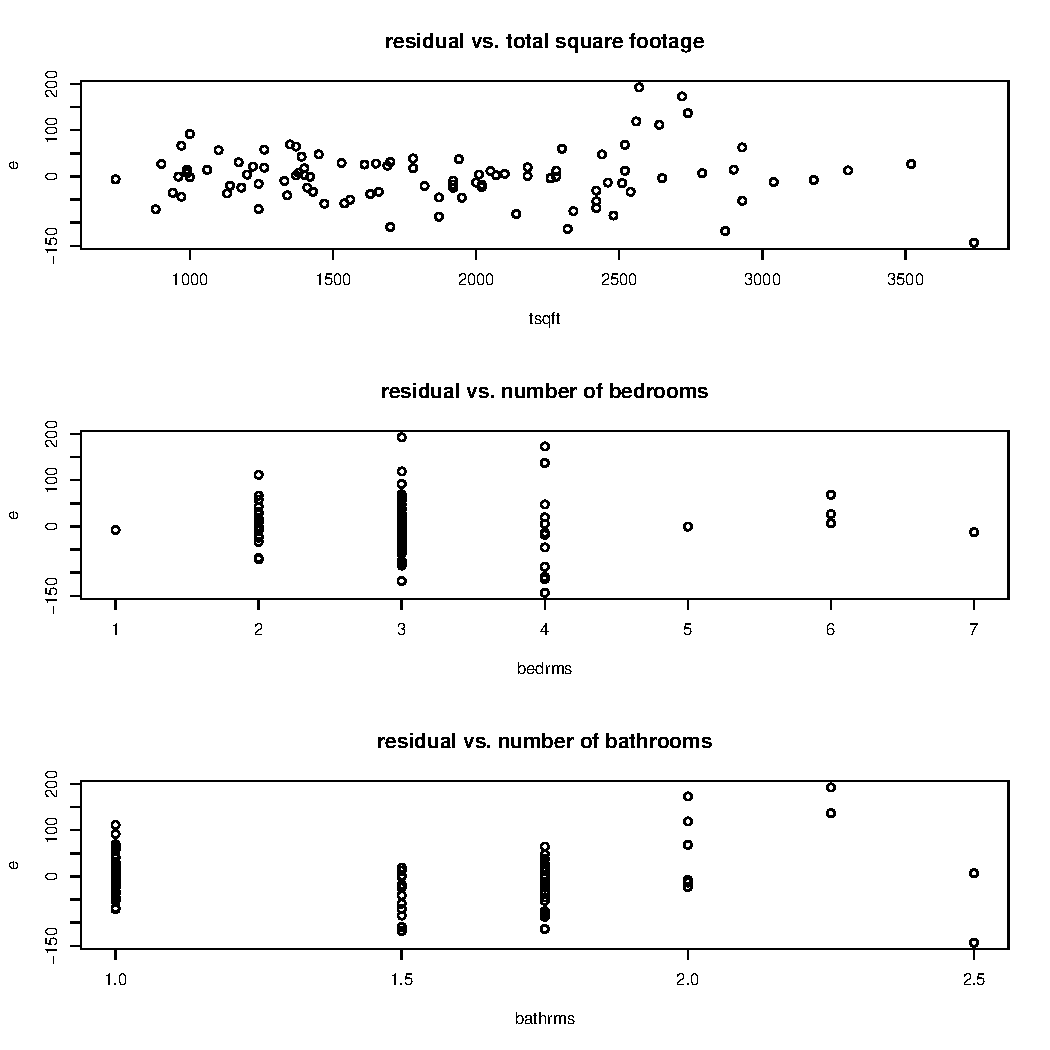
\includegraphics[width=\maxwidth]{figure/theme-R11-1} 

\end{knitrout}

The three residual-vs.-predictor plots are depicted for each of these predictors. It can be deduced that HSK exists for all three variables. There is strong HSK for \texttt{bedrms} and \texttt{bathrms} due to apparent increasing variance. For \texttt{tsqft}, HSK is not strong but we can further inspect this via tests.

\item Perform a Breusch-Pagan score test using the same three explanatory variables as HSK-driving suspects. Show the test results and state your test decision.

\begin{knitrout}
\definecolor{shadecolor}{rgb}{1, 1, 1}\color{fgcolor}\begin{kframe}
\begin{alltt}
\hlstd{int} \hlkwb{<-} \hlstd{(}\hlkwd{t}\hlstd{(e)} \hlopt \hlstd{e)} \hlopt{/} \hlstd{n}
\hlstd{g} \hlkwb{<-} \hlstd{(e} \hlopt{^} \hlnum{2} \hlopt{/} \hlstd{(int[}\hlnum{1}\hlstd{,} \hlnum{1}\hlstd{]))} \hlopt{-} \hlnum{1}
\hlcom{#capture variables you think may be related to HSK}
\hlstd{Z} \hlkwb{<-} \hlkwd{cbind}\hlstd{(}\hlkwd{rep}\hlstd{(n,} \hlnum{1}\hlstd{), tsqft}\hlopt{/}\hlnum{1000}\hlstd{, bedrms, bathrms)}
\hlstd{kz} \hlkwb{<-} \hlkwd{ncol}\hlstd{(Z)}
\hlstd{LM} \hlkwb{<-} \hlstd{(}\hlnum{1} \hlopt{/} \hlnum{2}\hlstd{)} \hlopt{*} \hlstd{(}\hlkwd{t}\hlstd{(g)} \hlopt \hlstd{Z} \hlopt \hlkwd{solve}\hlstd{(}\hlkwd{t}\hlstd{(Z)} \hlopt \hlstd{Z)} \hlopt \hlkwd{t}\hlstd{(Z)} \hlopt \hlstd{g)}
\hlstd{pval} \hlkwb{=} \hlnum{1} \hlopt{-} \hlkwd{pchisq}\hlstd{(LM, kz} \hlopt{-} \hlnum{1}\hlstd{)}
\end{alltt}
\end{kframe}
\end{knitrout}

The BP statistic for this test is 37.0887 and with degree of freedom equal to 3 it will result in the corresponding p-value of 0. That is we reject the null, implying the existence of HSK.

\item Then perform a White test, capture the results and state your test decision.  Make sure to include all \textit{permissible} interactions in your augmented data matrix.

\begin{knitrout}
\definecolor{shadecolor}{rgb}{1, 1, 1}\color{fgcolor}\begin{kframe}
\begin{alltt}
\hlstd{yaux} \hlkwb{<-} \hlstd{e} \hlopt{^} \hlnum{2} \hlcom{#use squared OLS residuals as dep.var. in White test}
\hlcom{#construct all permissible squared terms from the original X}
\hlstd{Xsq} \hlkwb{<-} \hlkwd{cbind}\hlstd{(bedrms} \hlopt{^} \hlnum{2}\hlstd{, bathrms} \hlopt{^} \hlnum{2}\hlstd{, distance} \hlopt{^} \hlnum{2}\hlstd{)}


\hlcom{#construct all permissible interaction terms from the original X}
\hlcom{# first for all continuous variables}
\hlstd{Xc1} \hlkwb{<-} \hlstd{tsqft}\hlopt{/}\hlnum{1000} \hlopt{*} \hlstd{bedrms}
\hlstd{Xc2} \hlkwb{<-} \hlstd{tsqft}\hlopt{/}\hlnum{1000} \hlopt{*} \hlstd{bathrms}
\hlstd{Xc3} \hlkwb{<-} \hlstd{tsqft}\hlopt{/}\hlnum{1000} \hlopt{*} \hlstd{distance}
\hlstd{Xc4} \hlkwb{<-} \hlstd{bedrms} \hlopt{*} \hlstd{bathrms}
\hlstd{Xc5} \hlkwb{<-} \hlstd{bedrms} \hlopt{*} \hlstd{distance}
\hlstd{Xc6} \hlkwb{<-} \hlstd{bathrms} \hlopt{*} \hlstd{distance}
\hlcom{#}
\hlcom{#next for the continuous with indicators}
\hlstd{dmat} \hlkwb{<-} \hlkwd{cbind}\hlstd{(garage, view)}
\hlstd{Xcitsqft} \hlkwb{<-} \hlkwd{matrix}\hlstd{(}\hlkwd{rep}\hlstd{(tsqft}\hlopt{/}\hlnum{1000}\hlstd{,} \hlnum{2}\hlstd{),} \hlkwc{nrow} \hlstd{= n)} \hlopt{*} \hlstd{dmat}
\hlstd{Xcibedrms} \hlkwb{<-} \hlkwd{matrix}\hlstd{(}\hlkwd{rep}\hlstd{(bedrms,} \hlnum{2}\hlstd{),} \hlkwc{nrow} \hlstd{= n)} \hlopt{*} \hlstd{dmat}
\hlstd{Xcibathrms} \hlkwb{<-} \hlkwd{matrix}\hlstd{(}\hlkwd{rep}\hlstd{(bathrms,} \hlnum{2}\hlstd{),} \hlkwc{nrow} \hlstd{= n)} \hlopt{*} \hlstd{dmat}
\hlstd{Xcidistance} \hlkwb{<-} \hlkwd{matrix}\hlstd{(}\hlkwd{rep}\hlstd{(distance,} \hlnum{2}\hlstd{),} \hlkwc{nrow} \hlstd{= n)} \hlopt{*} \hlstd{dmat}
\hlcom{#}
\hlcom{#Next: Run auxiliary regression and capture R^2}
\hlstd{Xaux} \hlkwb{<-}\hlkwd{cbind}\hlstd{(X,}
        \hlstd{Xsq,}
        \hlstd{Xc1,}
        \hlstd{Xc2,}
        \hlstd{Xc3,}
        \hlstd{Xc4,}
        \hlstd{Xc5,}
        \hlstd{Xc6,}
        \hlstd{Xcitsqft,}
        \hlstd{Xcibedrms,}
        \hlstd{Xcibathrms,}
        \hlstd{Xcidistance)}
\hlstd{kaux} \hlkwb{<-} \hlkwd{ncol}\hlstd{(Xaux)}
\hlstd{baux} \hlkwb{<-} \hlkwd{solve}\hlstd{((}\hlkwd{t}\hlstd{(Xaux))} \hlopt \hlstd{Xaux)} \hlopt \hlstd{(}\hlkwd{t}\hlstd{(Xaux)} \hlopt \hlstd{yaux)}
\hlstd{eaux} \hlkwb{<-} \hlstd{yaux} \hlopt{-} \hlstd{Xaux} \hlopt \hlstd{baux}
\hlstd{I} \hlkwb{<-} \hlkwd{diag}\hlstd{(n)}
\hlstd{i} \hlkwb{<-} \hlkwd{rep}\hlstd{(}\hlnum{1}\hlstd{, n)}
\hlstd{Mo} \hlkwb{<-} \hlstd{I} \hlopt{-} \hlstd{i} \hlopt \hlkwd{solve}\hlstd{(}\hlkwd{t}\hlstd{(i)} \hlopt \hlstd{i)} \hlopt \hlkwd{t}\hlstd{(i)}
\hlstd{SSE} \hlkwb{<-} \hlkwd{t}\hlstd{(eaux)} \hlopt \hlstd{eaux}
\hlstd{SST} \hlkwb{<-} \hlkwd{t}\hlstd{(yaux)} \hlopt \hlstd{Mo} \hlopt \hlstd{yaux}
\hlstd{R2} \hlkwb{<-} \hlnum{1} \hlopt{-} \hlstd{SSE} \hlopt{/} \hlstd{SST}
\hlstd{Wh} \hlkwb{<-} \hlstd{n} \hlopt{*} \hlstd{R2}
\hlstd{pval} \hlkwb{=} \hlnum{1} \hlopt{-} \hlkwd{pchisq}\hlstd{(Wh, kaux} \hlopt{-} \hlnum{1}\hlstd{)}
\end{alltt}
\end{kframe}
\end{knitrout}

The White statistic for this test is 51.8846 and with degree of freedom equal to 23 it will result in the corresponding p-value of \ensuremath{5\times 10^{-4}}. That is we reject the null, implying the existence of HSK.

\item Estimate a robust OLS model with White-corrected standard errors. Show your output.
\begin{knitrout}
\definecolor{shadecolor}{rgb}{1, 1, 1}\color{fgcolor}\begin{kframe}
\begin{alltt}
\hlstd{bols} \hlkwb{<-} \hlkwd{solve}\hlstd{((}\hlkwd{t}\hlstd{(X))} \hlopt \hlstd{X)} \hlopt \hlstd{(}\hlkwd{t}\hlstd{(X)} \hlopt \hlstd{y)}
\hlstd{e} \hlkwb{<-} \hlkwd{as.vector}\hlstd{(y} \hlopt{-} \hlstd{X} \hlopt \hlstd{bols)}
\hlstd{S} \hlkwb{<-} \hlkwd{diag}\hlstd{(e} \hlopt{^} \hlnum{2}\hlstd{)}
\hlstd{Vb} \hlkwb{<-} \hlkwd{solve}\hlstd{((}\hlkwd{t}\hlstd{(X))} \hlopt \hlstd{X)} \hlopt \hlkwd{t}\hlstd{(X)} \hlopt \hlstd{S} \hlopt \hlstd{X} \hlopt \hlkwd{solve}\hlstd{((}\hlkwd{t}\hlstd{(X))} \hlopt \hlstd{X)}
\hlstd{se_rols} \hlkwb{=} \hlkwd{sqrt}\hlstd{(}\hlkwd{diag}\hlstd{(Vb))}
\hlstd{tval_rols} \hlkwb{=} \hlstd{bols} \hlopt{/} \hlstd{se_rols}
\end{alltt}
\end{kframe}
\end{knitrout}

% latex table generated in R 3.6.2 by xtable 1.8-4 package
% Mon Apr 27 22:23:15 2020
\begin{table}[ht]
\centering
\caption{Robust OLS output} 
\begin{tabular}{lrrr}
  \hline
variable & estimate & s.e. & t \\ 
  \hline
constant & 17.62945 & 27.14990 & 0.64934 \\ 
  tsqft/1000 & 41.69129 & 9.57490 & 4.35423 \\ 
  bedrms & 26.83899 & 6.21989 & 4.31503 \\ 
  bathrms & 52.97844 & 19.20118 & 2.75912 \\ 
  garage & 23.51173 & 21.98210 & 1.06959 \\ 
  view & 83.57614 & 34.76247 & 2.40421 \\ 
  distance & -1.99078 & 0.49101 & -4.05443 \\ 
   \hline
\end{tabular}
\end{table}


\item Using the same HSK suspects, estimate your model through FGLS, using a multiplicative (don't forget the Harvey correction) form to model HSK.  Show your output.

\begin{knitrout}
\definecolor{shadecolor}{rgb}{1, 1, 1}\color{fgcolor}\begin{kframe}
\begin{alltt}
\hlcom{#Step 1: Consistent estimate of Omega}
\hlstd{yaux} \hlkwb{<-} \hlkwd{log}\hlstd{(e} \hlopt{^} \hlnum{2}\hlstd{)}
\hlstd{Xaux} \hlkwb{<-} \hlkwd{cbind}\hlstd{(}\hlkwd{rep}\hlstd{(n,} \hlnum{1}\hlstd{), tsqft}\hlopt{/}\hlnum{1000}\hlstd{, bedrms, bathrms)}
\hlstd{kaux} \hlkwb{<-} \hlkwd{ncol}\hlstd{(Xaux)}
\hlstd{baux} \hlkwb{<-} \hlkwd{solve}\hlstd{((}\hlkwd{t}\hlstd{(Xaux))} \hlopt \hlstd{Xaux)} \hlopt \hlstd{(}\hlkwd{t}\hlstd{(Xaux)} \hlopt \hlstd{yaux)}
\hlstd{sigvec} \hlkwb{<-} \hlkwd{as.vector}\hlstd{(}\hlkwd{exp}\hlstd{(Xaux} \hlopt \hlstd{baux)} \hlopt{+} \hlnum{1.2704}\hlstd{)} \hlcom{#Harvey's suggested correction}
\hlstd{Om} \hlkwb{<-} \hlkwd{diag}\hlstd{(sigvec)}
\hlcom{#}
\hlcom{#Step 2: GLS}
\hlstd{bgls} \hlkwb{<-} \hlkwd{solve}\hlstd{((}\hlkwd{t}\hlstd{(X))} \hlopt \hlkwd{solve}\hlstd{(Om)} \hlopt \hlstd{X)} \hlopt \hlstd{(}\hlkwd{t}\hlstd{(X)} \hlopt \hlkwd{solve}\hlstd{(Om)} \hlopt \hlstd{y)}
\hlstd{e} \hlkwb{<-} \hlstd{y} \hlopt{-} \hlstd{X} \hlopt \hlstd{bgls}
\hlstd{Vb} \hlkwb{<-} \hlkwd{solve}\hlstd{((}\hlkwd{t}\hlstd{(X))} \hlopt \hlkwd{solve}\hlstd{(Om)} \hlopt \hlstd{X)}
\hlstd{se_fgls} \hlkwb{=} \hlkwd{sqrt}\hlstd{(}\hlkwd{diag}\hlstd{(Vb))}
\hlstd{tval_fgls} \hlkwb{=} \hlstd{bgls} \hlopt{/} \hlstd{se_fgls}
\end{alltt}
\end{kframe}
\end{knitrout}

% latex table generated in R 3.6.2 by xtable 1.8-4 package
% Mon Apr 27 22:23:15 2020
\begin{table}[ht]
\centering
\caption{FGLS output} 
\begin{tabular}{lrrr}
  \hline
variable & estimate & s.e. & t \\ 
  \hline
constant & 16.44741 & 11.78645 & 1.39545 \\ 
  tsqft/1000 & 42.46043 & 4.15467 & 10.21994 \\ 
  bedrms & 25.87308 & 3.13223 & 8.26028 \\ 
  bathrms & 43.84951 & 7.21765 & 6.07531 \\ 
  garage & 40.07250 & 7.46697 & 5.36663 \\ 
  view & 87.83825 & 9.93626 & 8.84017 \\ 
  distance & -1.58775 & 0.19916 & -7.97206 \\ 
   \hline
\end{tabular}
\end{table}


\item Compare your original OLS estimates, the White corrected estimates, and the FGLS results and elaborate:

% latex table generated in R 3.6.2 by xtable 1.8-4 package
% Mon Apr 27 22:23:15 2020
\begin{table}[ht]
\centering
\caption{Comparison} 
\begin{tabular}{lrrrrrr}
  \hline
variable & s.e. (OLS) & s.e. (rOLS) & s.e. (FGLS) & t (OLS) & t (rOLS) & t (FGLS) \\ 
  \hline
constant & 31.00173 & 27.14990 & 11.78645 & 0.56866 & 0.64934 & 1.39545 \\ 
  tsqft/1000 & 10.03024 & 9.57490 & 4.15467 & 4.15656 & 4.35423 & 10.21994 \\ 
  bedrms & 7.46462 & 6.21989 & 3.13223 & 3.59549 & 4.31503 & 8.26028 \\ 
  bathrms & 17.51101 & 19.20118 & 7.21765 & 3.02544 & 2.75912 & 6.07531 \\ 
  garage & 20.39993 & 21.98210 & 7.46697 & 1.15254 & 1.06959 & 5.36663 \\ 
  view & 23.98448 & 34.76247 & 9.93626 & 3.48459 & 2.40421 & 8.84017 \\ 
  distance & 0.53391 & 0.49101 & 0.19916 & -3.72869 & -4.05443 & -7.97206 \\ 
   \hline
\end{tabular}
\end{table}


\begin{enumerate}[(a)]
\item Compare the s.e.’s and t-values between OLS and robust OLS. Are there any noteworthy changes in significance levels? In light of your finding, how does the naive OLS model mis-represent the significance of one or more coefficients?

\ksp
The t-values and standard errors are almost the same. The only difference is for the coefficient of \texttt{view} since its standard error is different between that of the OLS and robust OLS, the t-values are changing. This leads to different interpretations. For OLS, \texttt{view} iss statistically significant, but this is not the case for robust OLS.

\ksp
\item Compare the s.e.’s and t-values between the robust OLS and the FGLS model. Are there any noteworthy changes in significance levels?

\ksp
All the standard errors are smaller for FGLS. Since coefficient estimates are almost the same, this leads to significant estimates for all the variables of the FGLS model at both levels (1\% and 5\%). (t-values are larger for all coefficients in FGLS) However, for robust OLS, estimate for \texttt{Garage} is insignificant at both levels and \texttt{View} is only significant at 5\%.

\ksp
\item Assume the main focus of your research is on the effect of “view” and “distance” on home prices.  Overall, which model would you choose? (think: Are the gains in significance via FGLS worth the risk of misspecification bias? What about the sample size?).

\ksp
Even though the two methods will give us the same result for \texttt{Distance}, they give different results for \texttt{View}. (At least at 1\% significance level)

The Breusch-Pagan and White tests indicate the presence of HSK. We have two options: 1) ignoring the actual form or cause of HSK and choose robust OLS, or 2) assume a specific form of HSK and estimate a HSK-adjusted model via FGLS. In the case of the latter, if the assumption on the underlying form of HSK is incorrect, $\Omega$ will be misspecified, leading again to an inconsistent estimate. Therefore, we prefer to work with a less efficient but consistent robust model. Both FGLS and robust OLS are asymptotic methods. In our case we have a sample size of 100, hence we cannot merely rely on FGLS and/or robust OLS. 

At last, by taking into account all the aforementioned reasons, although the estimate given by FGLS (for these two variables) seem to be more precise and having smaller standard errors, we would prefer robust OLS.
\end{enumerate}

\end{enumerate}
\end{document}
